\section{Arquitetura Proposta}
\subsection{Descri��o}

\begin{figure}[tbh!]
	\centering
	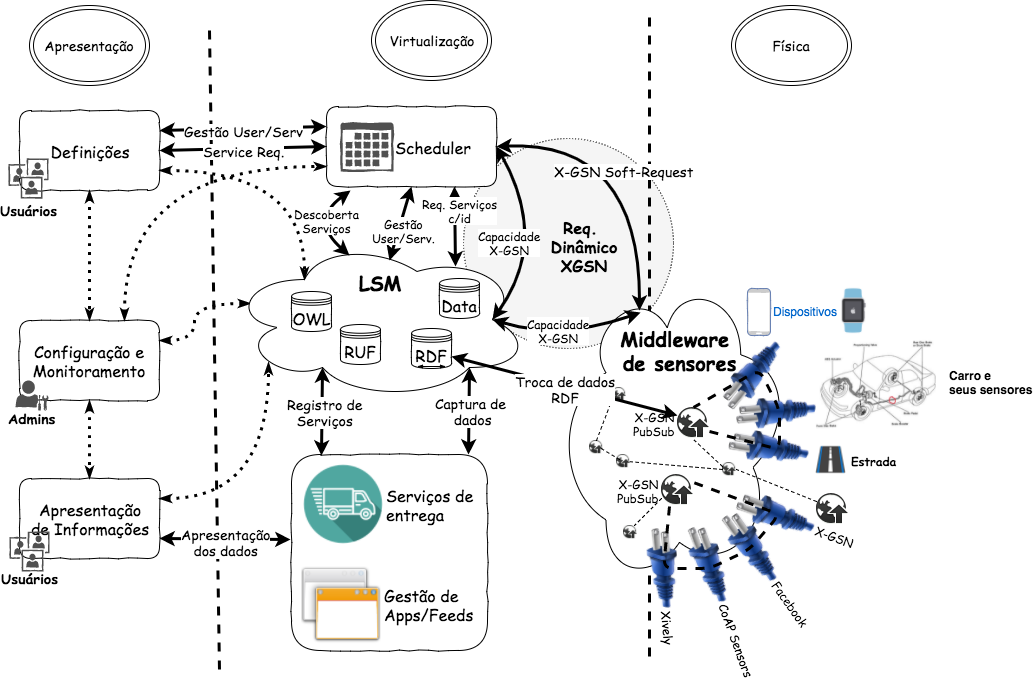
\includegraphics[width=1.0\textwidth]{../images/Ext_openIoTFull}
	\caption{Arquitetura do OpenIoT Full extendida}
	\label{fig:Ext_openIoTFull}
\end{figure}

\begin{figure}[tbh!]
	\centering
	\includegraphics[width=1.0\textwidth]{../images/Ext_openIoTLight}
	\caption{Arquitetura do OpenIoT Light extendida}
	\label{fig:Ext_openIoTLight}
\end{figure}

\begin{figure}[tbh!]
	\centering
	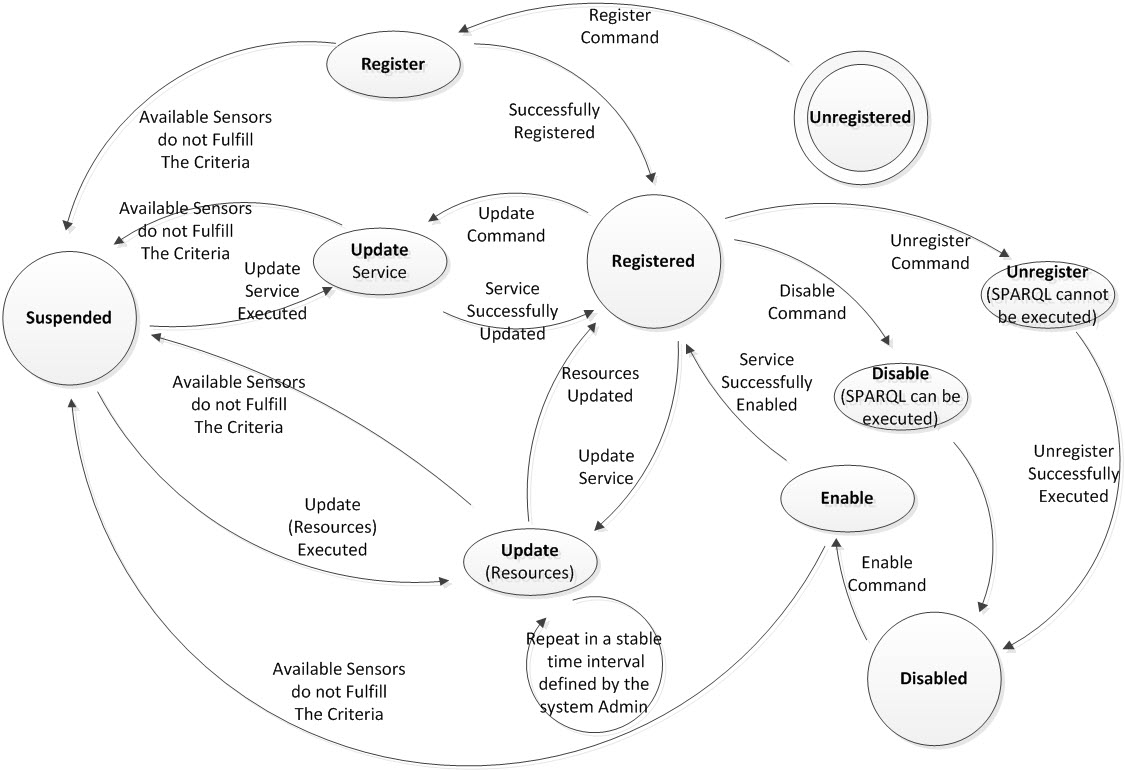
\includegraphics[width=1.0\textwidth]{../images/Ext_SchedulerServicesStateDiagram}
	\caption{Diagrama de Stados do Scheduler extendido}
	\label{fig:Ext_SchedulerServicesStateDiagram}
\end{figure}

\begin{figure}[tbh!]
	\centering
	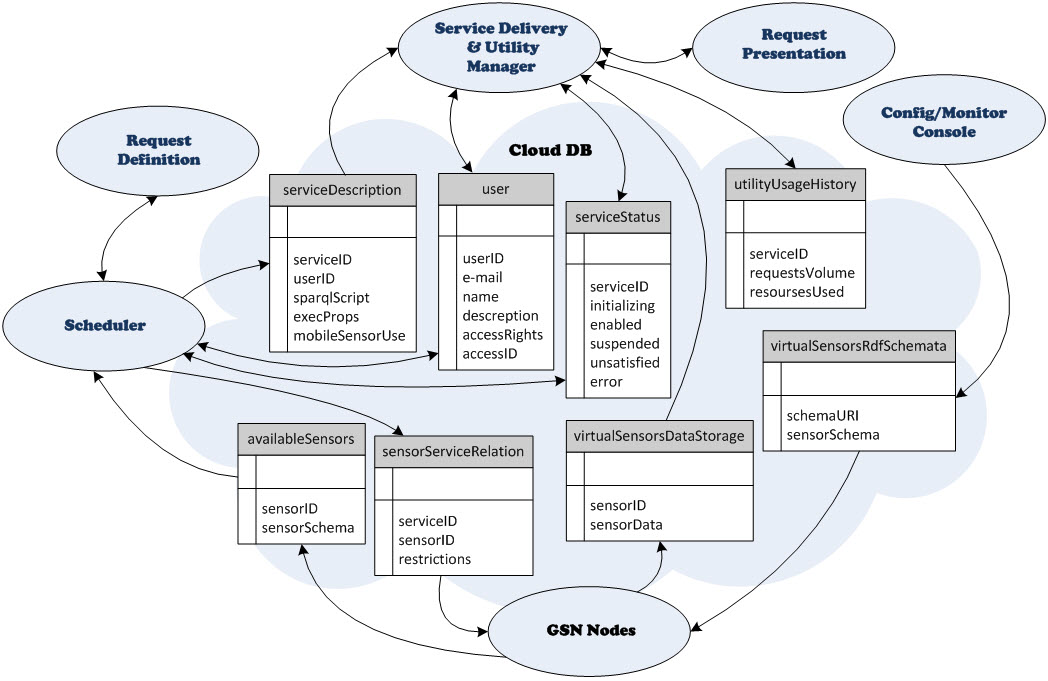
\includegraphics[width=1.0\textwidth]{../images/Ext_Architecture_DataAndRelationsWithoutStoringFormat}
	\caption{Relacionamento de dados extendido}
	\label{fig:Ext_Architecture_DataAndRelationsWithoutStoringFormat}
\end{figure}

\begin{figure}[tbh!]
	\centering
	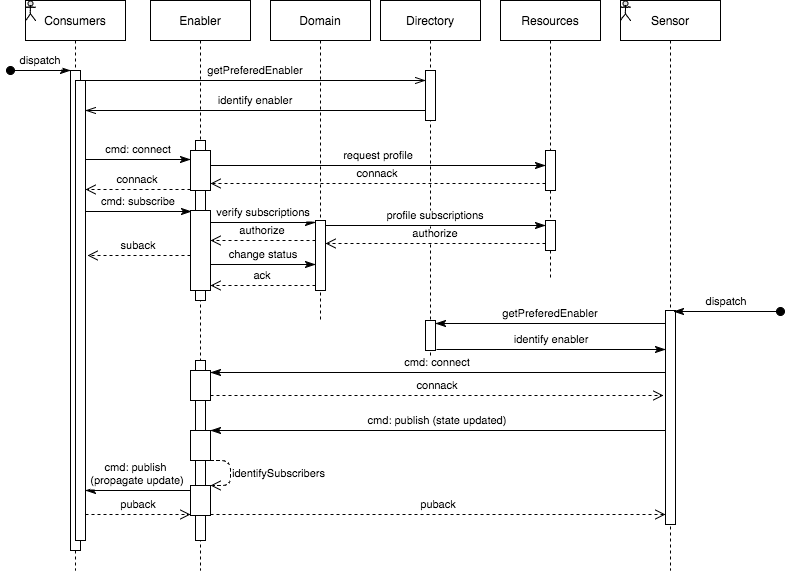
\includegraphics[width=1.0\textwidth]{../images/sequence1}
	\caption{Diagrama de sequ�ncia 1}
	\label{fig:sequence1}
\end{figure}

\begin{figure}[tbh!]
	\centering
	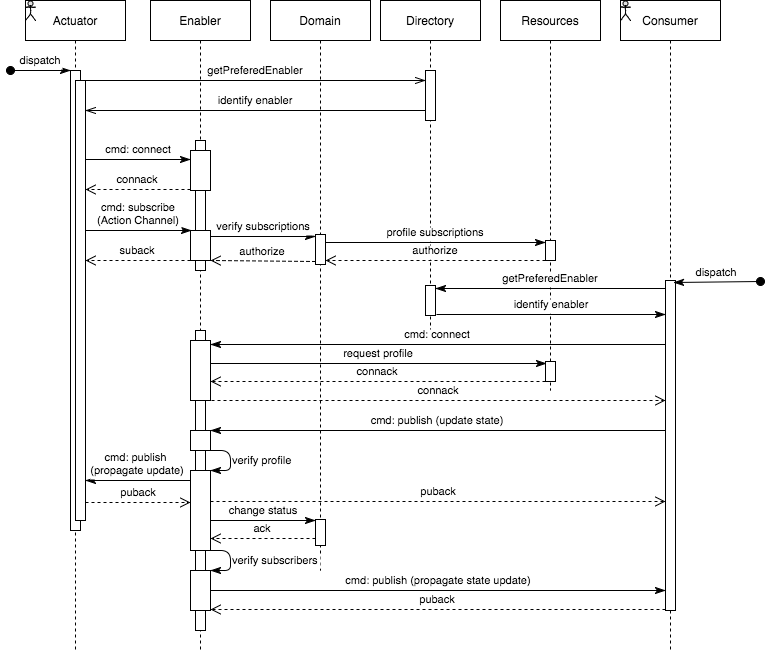
\includegraphics[width=1.0\textwidth]{../images/sequence2}
	\caption{Diagrama de sequ�ncia 2}
	\label{fig:sequence2}
\end{figure}

\begin{figure}[tbh!]
	\centering
	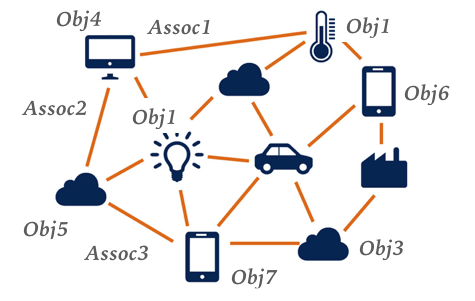
\includegraphics[width=1.0\textwidth]{../images/contexto}
	\caption{Exemplo de Contexto}
	\label{fig:contexto}
\end{figure}


\begin{figure}[tbh!]
	\centering
	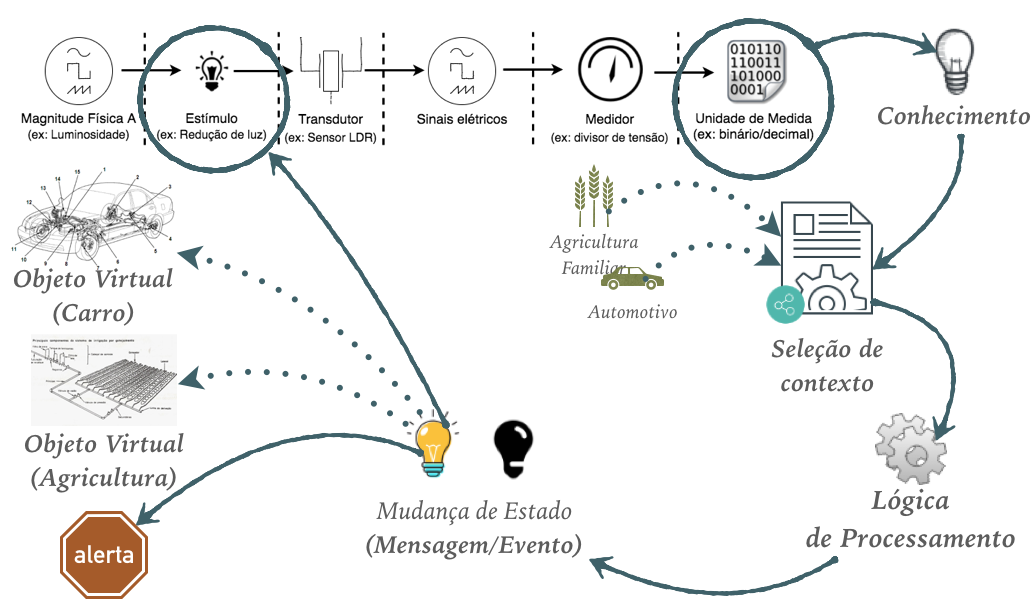
\includegraphics[width=1.0\textwidth]{../images/ciclodeconhecimento}
	\caption{Representa��o do ciclo do Conhecimento}
	\label{fig:ciclodeconhecimento}
\end{figure}

\begin{figure}[tbh!]
	\centering
	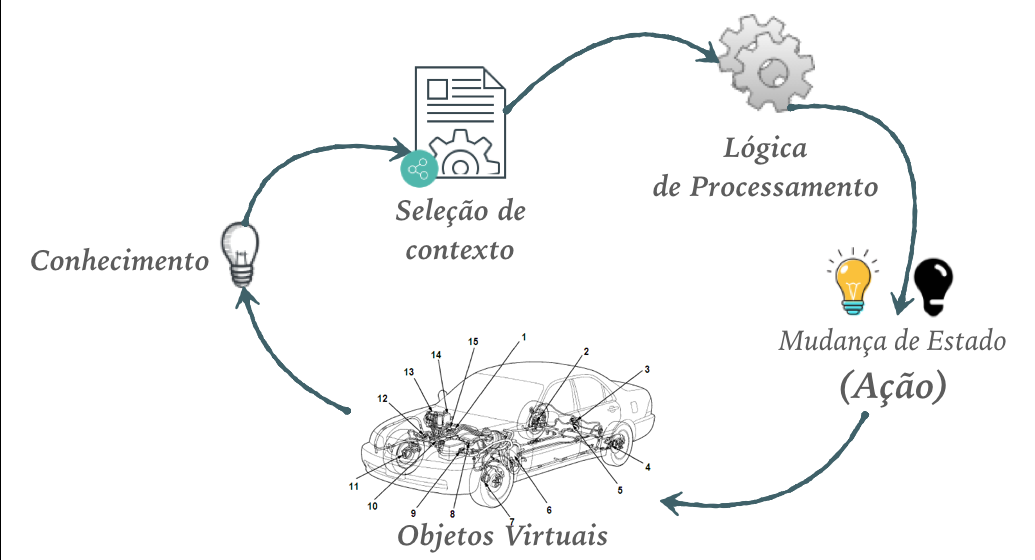
\includegraphics[width=1.0\textwidth]{../images/ciclodevidaobjetos}
	\caption{Ciclo de Vida dos Objetos Virtuais}
	\label{fig:ciclodevidaobjetos}
\end{figure}


\begin{figure}[tbh!]
	\centering
	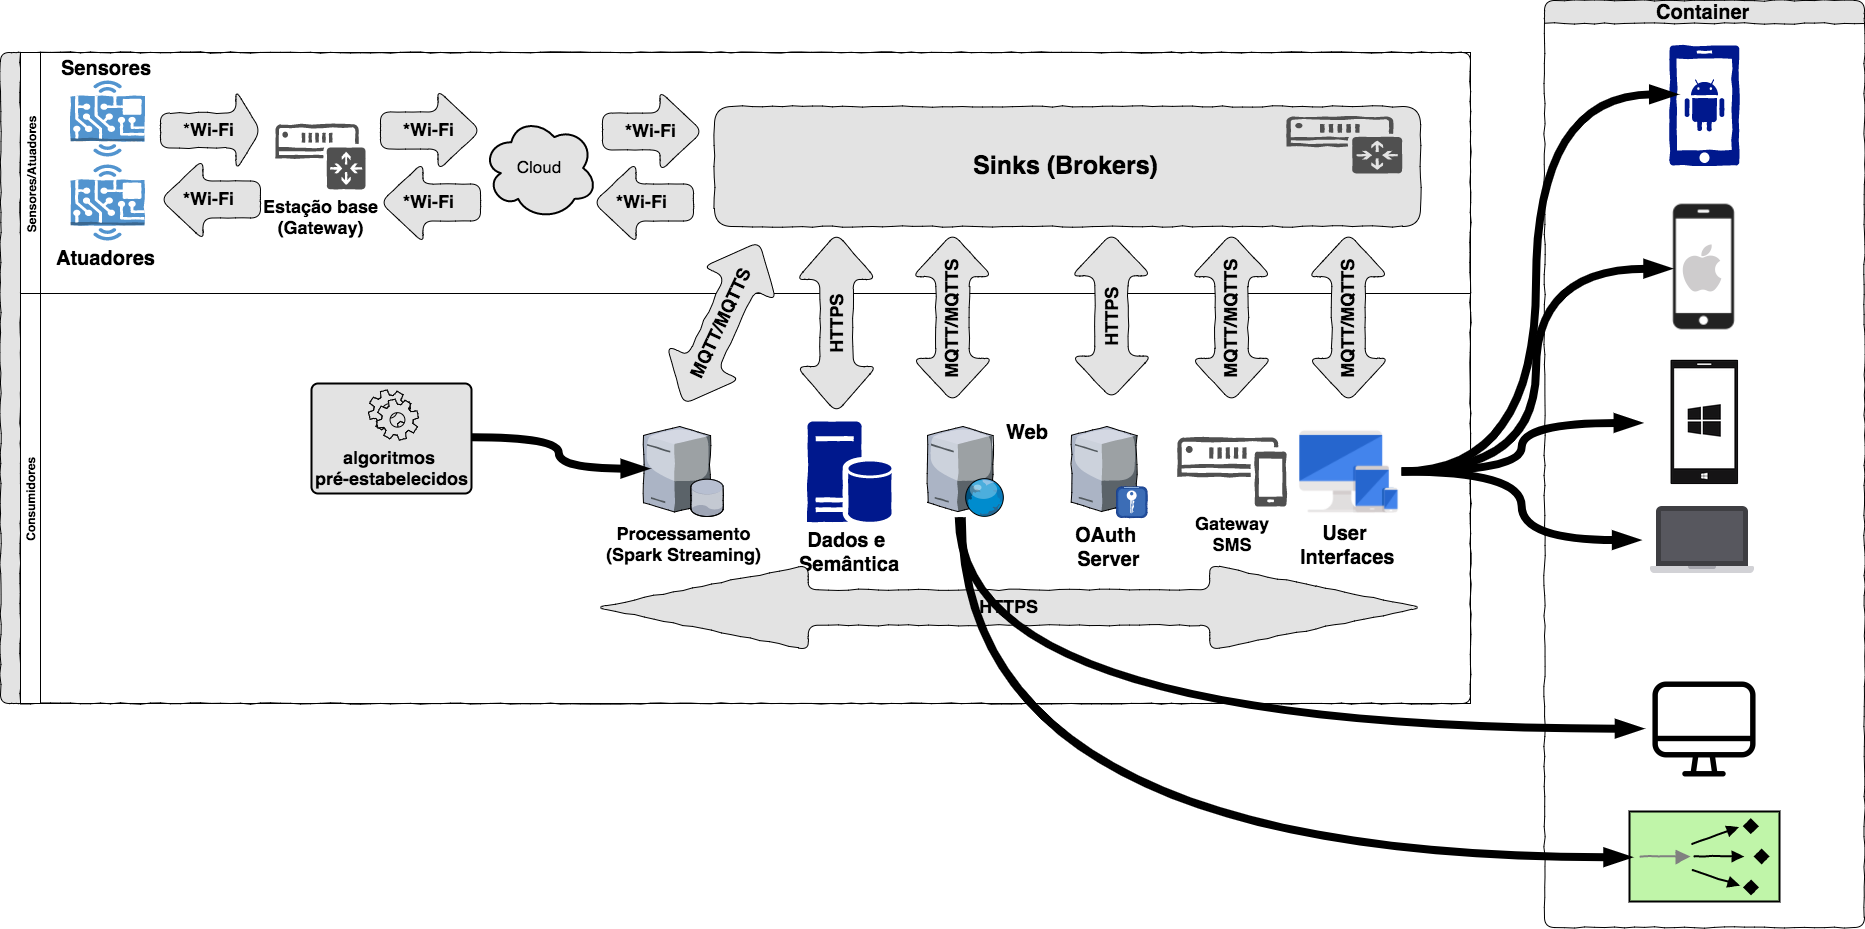
\includegraphics[width=1.0\textwidth]{../images/arquitetura_rede}
	\caption{Arquiteteura 2}
	\label{fig:arquitetura2}
\end{figure}